\documentclass[12pt, a4paper]{article}
\usepackage[margin=0.7in]{geometry}

\usepackage[none]{hyphenat}

\usepackage{bookmark}
\usepackage{adjustbox}
\usepackage{mathtools}
\usepackage{amsmath}
\usepackage{amssymb}
\usepackage{amsthm}
\usepackage{amsfonts}
\usepackage{algorithmic}

\usepackage{pgfplots}
\pgfplotsset{compat=1.16}
\usepackage{tikz}
\usetikzlibrary{arrows}
\usepackage{graphicx}
\usepackage{pst-solides3d}
\usepackage{xcolor}
\usepackage{hyperref}
\usepackage[cache=false]{minted}

\usepackage{soul}
\usepackage{cite}
\usepackage{textcomp}

\usepackage{wasysym}

% Sets and related operations
\newcommand{\nats}{\mathbb{N}} % Natural numbers
\newcommand{\pnats}{\mathbb{N}^+} % Positive natural numbers

\newcommand{\ints}{\mathbb{Z}} % Integers
\newcommand{\pints}{\mathbb{Z}^+} % Positive integers
\newcommand{\nints}{\mathbb{Z}^-} % Negative integers

\newcommand{\rats}{\mathbb{Q}} % Rational numbers
\newcommand{\prats}{\mathbb{Q}^+} % Positive rational numbers
\newcommand{\nrats}{\mathbb{Q}^-} % Negative rational numbers

\newcommand{\reals}{\mathbb{R}} % Real numbers
\newcommand{\preals}{\mathbb{R}^+} % Positive real numbers
\newcommand{\nreals}{\mathbb{R}^-} % Negative real numbers

\newcommand{\irrats}{\mathbb{I}} % Irrational numbers


\newcommand{\pset}{\mathcal{P}} % Powerset
\newcommand{\card}{\abs} % Cardinality
\newcommand{\topology}{\mathcal{T}} % Topology
\newcommand{\basis}{\mathcal{B}} % Basis

% Calligraphy
\newcommand\und[1]{\underline{\smash{#1}}}

% Operators
\DeclarePairedDelimiter\abs{\lvert}{\rvert}
\DeclarePairedDelimiter\ceil{\lceil}{\rceil}
\DeclarePairedDelimiter\floor{\lfloor}{\rfloor}

% Other
\newcommand{\rarr}{\rightarrow}
\newcommand{\larr}{\leftarrow}

% Setting stuff
\setlength{\parindent}{0pt}


% Title
\title{\rule{\paperwidth - 150pt}{1pt}\textbf{\\\textit{Topology}\\}\rule{\paperwidth - 150pt}{1pt}}

\author
{
Author: David Oniani\\
Instructor: Dr. Eric Westlund
}

\date{January 13, 2019}


\begin{document}
\maketitle

\center{\Large Assignment \textnumero{2}}

\begin{itemize}
\item[]
\item[]
{\large \textbf{Section 13}}
\vspace{0.3cm}

% Begin here!

\item[7.]
Consider the following topologies on $\reals$:
\begin{align*}
&\topology_1 = \mbox{the standard topology,}\\
&\topology_2 = \mbox{the topology of }\reals_K,\\
&\topology_3 = \mbox{the finite complement topology,}\\
&\topology_4 = \mbox{the upper limit topology, having all sets }(a, b] \mbox{ as basis,}\\
&\topology_5 = \mbox{the topology having all sets }(-\infty, a] = \{x \ | \ x < a\} \mbox{ as basis.}\\
\end{align*}
Determine, for each of these topologies, which of the other it contains.
\begin{quote}
From \textbf{Lemma 13.4}, we know that $\topology_2$ is strictly finer than $\topology_1$.
\newline
\newline
The finite complement topology will look like $(-\infty, x_0) \ \cup \ (x_0, x_1) \ \cup .... (x_{n - 1}, +\infty)$.
Then it is easy to notice that $\topology_1$ is strictly finer than $\topology_3$ (since $\topology_3$ is an open set in $\topology_1$; also $(2, 3)$ is open in standard topology but not in finite complement topology).
\newline
\newline
Now, let $B = (a, b)$ be the element in the basis of $\topology_1$. Let $x \in B$. Then, we can
find element $(a, x]$ in the upper limit topology that clearly contains element $x$. Hence, the upper limit
topology is finer standard topology. In fact $\topology_4$ is strictly finer than $\topology_1$ since $(2, 3]$
is not open in $\topology_1$.
\newline
\newline
Hence, as of now, we have the relationship $\topology_3 \subsetneq \topology_1 \subsetneq \topology_2, \topology_4$.
\newline
\newline
Let's now find out the relationship between $\topology_2$ and $\topology_4$.
\newline
\newline
The upper limit topology is finer than the topology of $\reals_K$.\ To show this let
$B = (a, b) - K$ be the element in the basis of $\topology_2$.\ Then let $x \in B$.
If $x < 0$, then we can find element $(a, x]$ which is in the basis of the $\topology_4$.
In this case, it is easy to notice that $x \in (a, x] \in B$. On the other hand, if $x \geq 0$,
then let $k$ be the smallest integer such that $\frac{1}{k} < x$. We have $B \cap (\frac{1}{n}, x] = (s, x]$
where $s = a$ if $a > \frac{1}{k}$ and $s = \frac{1}{k}$ if $\frac{1}{k} > a$. It follows that
$x \in (s, x] \subset B$, and we get that $(x, s]$ is a basis element for $\topology_4$.
Hence, we got that $\topology_2 \subset \topology_4$.
\newline
\newline
Now our relationship looks a bit better: $\topology_3 \subsetneq \topology_1 \subsetneq \topology_2 \subset \topology_4$.
\newline
\newline
Let's now find the relationship between $\topology_5$ and $\topology_1$.\
Let $B = (-\infty, a]$ the element in the basis for $\topology_5$.
Then let $x \in B$. Notice that $B = \bigcup_{i = 1}^{+\infty}(-i, a)$.
Knowing that any topology is closed under union, we then know that $B \in \topology_1$.
Thus, we got that $\topology_5 \subset \topology_1$. Now, notice that there is no element $e$
such that $e \in (-\infty, 2) \subset (2, 3)$ hence, $\topology_1$ is strictly finer than $\topology_5$
and $\topology_5 \subsetneq \topology_1$.
\newline
\newline
As of now, our relationship is $\topology_3, \topology_5 \subsetneq \topology_1 \subsetneq \topology_2 \subset \topology_4$.
\newline
\newline
Finally, let's find out the relationship between $\topology_3$ and $\topology_5$.
They are not comparable! (I looked at the previous exercise which asks for similar but not exactly the same question/proof -- \textbf{Exercise 6}).
Consider two open sets $\reals - \{2\}$ and $(-\infty, 4)$ from $\topology_3$ and $\topology_5$ correspondingly.
Then both open sets contain the point $3$, however, neither of these open sets contain
the open set from the other topology that contains $3$. Hence, there is no way to find out whether
$\topology_3$ is finer than $\topology_5$, vice versa.
\newline
\newline
Finally, we have established the relationship $\topology_3, \topology_5 \subsetneq \topology_1 \subsetneq \topology_2 \subset \topology_4$
with $\topology_3$ and $\topology_5$ being impossible to compare.
\end{quote}

\item[]
\item[]

\item[8.]
\begin{itemize}
\item[(a)]
Apply Lemma 13.2 to show that the countable collection
$$\basis = \{(a, b) \ | \ a < b, a \mbox{ and } b \mbox{ rational} \}$$
is a basis that generates the standard topology on $\reals$.
\begin{quote}
Suppose that $(c, d)$ is the element in the basis of the standard topology.
Let $x \in (c, d),\  c < x < d$. Then $\exists a, b \in \rats$ such that $c < a < x < b < d$.
Below is the graphical representation of how the sets would look like
(it is obviously not necessary, just learning how to to use the \texttt{tikz}
package {\Large\smiley}).

\item[]
\item[]

\begin{center}
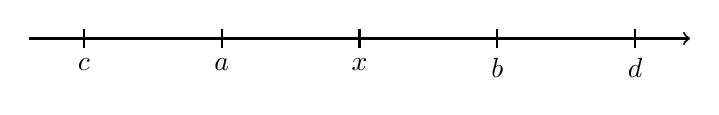
\begin{tikzpicture}[scale=7]
    \draw[->, thick] (-0.1,0) -- (1.1,0);
    \foreach \x/\xtext in {0/$c$,0.25/$a$,0.5/$x$,0.75/$b$,1/$d$}
        \draw[thick] (\x,0.5pt) -- (\x,-0.5pt) node[below] {\xtext};
\end{tikzpicture}
\end{center}

\item[]
\item[]

We got $x \in (a, b) \subset (c, d)$ with $(c, d) \in \basis$.
In other words, $\forall x \in B_{\reals}$ (where $B_{\reals}$ is the open
set of $\reals$), $\exists C$ such that $x \in C \subset B_{\reals}$.
We can now apply $\textbf{Lemma 13.2}$ and claim that $\basis$ is the basis
that generates the standard topology on $\reals$.$\qed$
\end{quote}

\newpage

\item[(b)]
Show that the collection
$$\mathcal{C} = \{[a, b) \mid a < b, a \mbox{ and } b \mbox{ are rational}\}$$
is a basis that generates a topology diffferent from the lower limit topology on $\reals$.
\begin{quote}
Consider the point $\sqrt{5}$ in the open
set $[\sqrt{5}, 5)$ of the lower limit topology. Then, since $\mathcal{C}$ can only generate
open sets of the topology of the type $(a, b)$ where $a < b \ \wedge a, b \in \rats$ or unions
of such sets, it is clear that there is no basis element in $\mathcal{C}$
which would contain $\sqrt{5}$ and be a subset of $[\sqrt{5}, 5)$.
In fact, the topology generated by $\mathcal{C}$ is strictly coarser than
the lower limit topology on $\reals$.$\qed$
\end{quote}
\end{itemize}

\item[]
\item[]
\item[]

{\large \textbf{Section 16}}
\vspace{0.3cm}
\item[3.]
Consider the set $Y = [-1, 1]$ as a subspace of $\reals$.
Which of the following sets are open in $Y$? Which are open in $\reals$?
\begin{align*}
&A = \{x \mid \frac{1}{2} < \abs{x} < 1\},\\
&B = \{x \mid \frac{1}{2} < \abs{x} \leq 1\},\\
&C = \{x \mid \frac{1}{2} \leq \abs{x} < 1\},\\
&D = \{x \mid \frac{1}{2} \leq \abs{x} \leq 1\},\\
&E = \{x \mid 0 < \abs{x} < 1 \ \mbox{and} \ 1/x \notin \pints\}.
\end{align*}
\begin{quote}
Let's check the openness in $Y$ and $\reals$ one by one.
\newline
\newline
First consider the set $A = \{x \mid \frac{1}{2} < \abs{x} < 1\}$.
Notice that $A$ is the union of open intervals since is open in $\reals$.
Because $Y \subset \reals$, $A$ is also open in $Y$.
\newline
\newline
Consider the set $B = \{x \mid \frac{1}{2} < \abs{x} \leq 1\}$.
We have $1 \in B$, but for any $\delta > 0$, $(1, \delta) \not\subset B$.
Hence, $B$ is not open in $\reals$. Now notice that $B = Y \ \cap \ ((-2, -\frac{1}{2}) \cup (\frac{1}{2}, 2)) = [-1, -\frac{1}{2}) \ \cup \ (\frac{1}{2}, 1]$.
Now, since, $[-1, -\frac{1}{2}) \ \cup \ (\frac{1}{2}, 1]$ is open, $B$ is open in $Y$.
\newline
\newline
Now, let's take a look at the set $C = \{x \mid \frac{1}{2} \leq \abs{x} < 1\}$.
Suppose, for the sake of contradiction, that $C$ is open in $Y$.
Then $\exists U \in Y$ such that $C = U \cap Y$. In other words,
$\exists \delta > 0$ such that $(\frac{1}{2}, \delta) \in U$.
Then there would also exist $\delta\prime$ such that $(\frac{1}{2}, \delta\prime) \in C$
which is false. Thus, we have reached the contradiction and the set $C$
is not open in $Y$. It follows that $C$ is also not open in $\reals$.
\newline
\newline
Consider the set $D = \{x \mid \frac{1}{2} \leq \abs{x} \leq 1\}$.
Suppose, for the sake of contradiction, that $D$ is open in $Y$.
Then $\exists U \in Y$ such that $D = U \cap Y$. In other words,
$\exists \delta > 0$ such that $(\frac{1}{2}, \delta) \in U$.
Then there would also exist $\delta\prime$ such that $(\frac{1}{2}, \delta\prime) \in D$
which is false. Thus, we have reached the contradiction and the set $D$
is not open in $Y$. It follows that $D$ is also not open in $\reals$.
\newline
\newline
$E$ is open in both $Y$ and $\reals$ since it is the union of open intervals.
\newline
\newline
Finally, we got that $A$ and $E$ are open in both $Y$ and $\reals$.
The set $B$ is open only in $Y$. And sets $C$ and $D$ are not open in $Y$ or $\reals$.
\end{quote}

\item[]
\item[]

\item[4.]
A map $f : X \rarr Y$ is said to be an \textbf{open map} if for every open set $U$ of $X$,
the set $f(U)$ is open in $Y$. Show that $\pi_1 : X \times Y \rarr X$ and $\pi_2 : X \times Y \rarr Y$ are open maps.
\begin{quote}
At first, let us show that $\pi_1 : X \times Y \rarr X$ is an open map.
Let $U \subset X \times Y$ be an open set and let $x \in \pi_1(U)$. Then $\exists y$ such that $x \times y \in U$.
Now, because $U$ is open, there is a basis set $A \times B \in U$ such that $x \times y \in U$.
Now, since $A \times B$ is a basis set, $A$ is open in $X$. Besides, $x \in A = \pi_1(A \times B) \subset \pi_1(U)$.
Hence, $\pi_1(U)$ is open. Therefore, $\pi_1 : X \times Y \rarr X$ is an open map.$\qed$
\newline
\newline
Now, let's show that $\pi_2 : X \times Y \rarr Y$ is an open map.
Let $V \subset X \times Y$ be an open set and let $y \in \pi_1(V)$. Then $\exists x$ such that $x \times y \in V$.
Now, because $V$ is open, there is a basis set $A \times B \in V$ such that $x \times y \in V$.
Now, since $A \times B$ is a basis set, $B$ is open in $Y$. Besides, $y \in B = \pi_1(A \times B) \subset \pi_1(V)$.
Hence, $\pi_2(V)$ is open. Therefore, $\pi_2 : X \times Y \rarr Y$ is an open map.$\qed$
\end{quote}

\item[]
\item[]

\item[6.]
Show that the countable collection
$$\{(a, b) \times (c, d) \mid a < b \mbox{ and } c < d, \mbox{and } a,b,c,d \mbox{ are rational}\}$$
is a basis for $\reals^2$.
\begin{quote}
For simplicity, let's call this set $S$. Thus, $S = \{(a, b) \times (c, d) \mid a < b \mbox{ and } c < d, \mbox{and } a,b,c,d \mbox{ are rational}\}$.
\newline
\newline
Suppose that $(a, b) \times (c, d)$ is the element in the basis of the topology for $\reals^2$. Let $x \in (a, b) \times (c, d)$.
Then $\exists e, f, g, h \in \rats$ with $e < f$ and $g < h$ such that $(e, f) \times (g, h) \subset (a, b) \times (c, d)$.
In other words, $\forall x \in B_{\reals^2}$ (where $B_{\reals^2}$ is the open set in $\reals^2$), $\exists C$ such that
$x \in C \subset B_\reals^2$. We can now apply $\textbf{Lemma 13.2}$ and claim that $S$ is the basis that generates the topology on $\reals^2$.$\qed$
\end{quote}

\item[]
\item[]

\item[10.]
Let $I = [0, 1]$. Compare the product topology on $I \times I$, the dictionary order
topology on $I \times I$, and the topology $I \times I$ inherits the subspace of $\reals \times \reals$
in the dictionary order topology.
\begin{quote}
Let's first compare the product topology on $I \times I$ and the dictionary order topology on $I \times I$.
Notice that the dictionary order topology and the product topology are strictly contained in the subspace
topology from the dictionary order on the plane, and hence are incomparable with one another.
\newline
\newline
CONTINUE HERE!
\end{quote}

\item[]
\item[]
\item[]

{\large \textbf{Section 17}}
\vspace{0.3cm}
\item[3.]
Show that if $A$ is closed in $X$ and $B$ is closed in $Y$, then $A \times B$ is closed in $X \times Y$.
\begin{quote}
Notice that $A \times B = X \times Y - (((X - A) \times Y) \cup (X \times (Y - B)))$.
Since $A$ is closed in $X$, $X - A$ is open in $X$ and thus $(X - A) \times Y$ is open in $X \times Y$.
Similarly, since $B$ is closed in $Y$, $Y - B$ is open in $Y$ and therefore $X \times (Y - B)$ is open in $X \times Y$.
Then we have that $((X - A) \times Y) \cup (X \times (Y - B))$ is open and hence $X \times Y - ((X - A) \times Y) \cup (X \times (Y - B))$
is closed. Finally, $A \times B$ is closed in $X \times Y$.$\qed$
\end{quote}

\item[]
\item[]

\item[6.]
Let $A, B,$ and $A_\alpha$ denote subsets of a space $X$. Prove the following:
\begin{itemize}
\item[(a)]
If $A \subset B$, then $\bar{A} \subset \bar{B}$.
\begin{quote}
Suppose that $A, B \subset X$ and $A \subset B$.
\end{quote}
\end{itemize}

\item[]
\item[]

\item[11.]
Show that the product of two Hausdorff spaces are Hausdorff.
\begin{quote}
To prove that the product of two Hausdorff spaces are Hausdorff,
it is sufficient to show that $\forall x_1, x_2$ such that $x_1 \neq x_2$,
$\exists U_1, U_2$ of $x_1$ and $x_2$ respectively with $U_1 \cap U_2 = \emptyset$ ($U_1, U_2$ are neighborhoods).
Suppose we have two Hausdorff spaces $X$ and $Y$.
Let $x_1, x_2 \in X$. Then $\exists U_1, U_2 \subset X$
such that $U_1 \cap U_2 = \emptyset$. Now consider the sets
$V_1 = U_1 \times Y$ and $V_2 = U_2 \times Y$. Notice that
$V_1 \cap V_2 = (U_1 \cap U_2) \times Y = \emptyset \times Y = \emptyset$.
Thus, we got that $X \times Y$ is Hausdorff.$\qed$
\end{quote}

\item[]
\item[]

\item[16.]
Consider the five topologies on $\reals$ given in Exercise 7 of §13.
\begin{itemize}
\item[(a)]
Determine the closure of the set $K = \{1/n \mid n \in \pints\}$ under each of these topologies.
\begin{quote}
Let's consider each of these topologies one by one.
\item[]
\item[]
\begin{itemize}
\item[1.]
$\topology_1 = \mbox{ the standard topology.}$
\begin{quote}
Let $x < 0$. Then notice that $(\frac{5x}{4}, \frac{x}{2})$
is an open neighborhood of $x$ that has no intersection
with $K$. Now, since $K \subset \bar{K}$, it follows that $x \notin \bar{K}$. Now consider the case when $x > 1$.
Notice that open set $(x + \frac{1 - x}{2}, x - \frac{1 - x}{2})$ is a neighborhood of $x$ that does not intersect $K$.
Therefore, since $K \subset \bar{K}$, it follows that $x \notin \bar{K}$. If $x \in (0, 1)$. Then notice that $\exists l \in \pints$ such that $\frac{1}{l + 1} < x < \frac{1}{l}$.
Then this neighborhood has no intersection with $K$ and therefore, $x \notin \bar{K}$. We are now left with point $0$.
Suppose that $U$ is an open neighborhood of $0$. Then there
exists the basis element $0 \in (a, b) \subset U$. In fact,
there must exist $m \in \pints$ such that $\frac{1}{m} < b$
with $\frac{1}{m} \in U \cap K$. The notice that $U \cap K$
is non-empty for any neighborhood $U$ of 0. Therefore, $0 \in \bar{K}$. Finally, $\bar{K} = \{0\}$

\end{quote}

\item[]

\item[2.]
$\topology_2 = \mbox{ the topology of $\reals_K$.}$
\begin{quote}
In the topology of $\reals_K$, $\reals - K$ is considered open.
Thus, $K$ is closed and, according to \textbf{Theorem 17.6}, $\bar{K} = K + \emptyset = K$.
Therefore, the closure of the set $K$ is $K$.
\end{quote}

\item[]

\item[3.]
$\topology_3 = \mbox{ the finite complement topology.}$
\begin{quote}
Notice that in the finite complement topology,
every closed set is either finite or all of $\reals$.
Then obviously infinite set $K$ cannot be a subset of any finite set
and it follows that $\reals$ must be the only closed set that contains $K$.
Therefore, $\bar{K} = \reals$.
\end{quote}

\item[]

\item[4.]
$\topology_4 = \mbox{ the upper limit topology, having all sets $(a, b]$ as basis.}$
\begin{quote}
Consider the set $\reals - K$. Notice that $\reals - K = (-\infty, 0] \cup \bigcup_{i \in \pints}(\frac{1}{i + 1}, \frac{1}{i}) \cup (1, +\infty)$.
Then $\forall U \in \reals - K$, $U$ is open in the upper limit topology and hence, $\reals - K$ is open.
Therefore, $K$ is closed and $\bar{K} = K$.
\end{quote}

\item[]

\item[5.]
$\topology_5 = \mbox{the topology having all sets }(-\infty, a] = \{x \ | \ x < a\} \mbox{ as basis.}$
\begin{quote}
Let $x < 0$, then $(-\infty, x]$ has no intersections with $K$, hence $x \notin \bar{K}$. Now let $x \geq 0$. Then
all neighborhoods of $x$ contain a basis set $(-\infty, y)$
where $y > 0$. Let $U$ be a neighborhood of $x$. Then $\exists z$ such that $\frac{1}{z} < y$. Therefore, $\frac{1}{z} \in U \cup K$. Finally, $x \in \bar{K}$ and $\bar{K} = [0, +\infty)$.
\newline
\newline
To summarize, we got that the closure of $K$ under $\topology_1$ is $\{0\}$, under $\topology_2$ is $K$, under
$\topology_3$ is $\reals$, under $\topology_4$ is $K$,
and under $\topology_5$ is $[0, +\infty)$.
\end{quote}
\end{itemize}
\end{quote}

\item[]
\item[]

\item[(b)]
Which of these topologies satisfy the Hausdorff axiom? the $T_1$ axiom?
\begin{quote}
Once again, let's go through all of the topologies one at a time.
\begin{itemize}
\item[1.]
$\topology_1 = \mbox{ the standard topology.}$
\begin{quote}
Notice that $\forall x, y$ such that $x \neq y$, $x \in (x - \frac{{\abs{x - y}}}{2}, x + \frac{{\abs{x - y}}}{2})$
and $y \in (y - \frac{{\abs{x - y}}}{2}, y + \frac{{\abs{x - y}}}{2})$. Besides, $(x - \frac{{\abs{x - y}}}{2}, x + \frac{{\abs{x - y}}}{2}) \cap (y - \frac{{\abs{x - y}}}{2}, y + \frac{{\abs{x - y}}}{2}) = \emptyset$. Hence, the standard
topology is both Hausdorff and $T_1$.
\end{quote}

\item[]

\item[2.]
$\topology_2 = \mbox{ the topology of $\reals_K$.}$
\begin{quote}
We know that the topology on $\reals_K$ is finer than
the standard topology. This is sufficient to say that
it is both Hausdorff and $T_1$.
\end{quote}

\item[]

\item[3.]
$\topology_3 = \mbox{ the finite complement topology.}$
\begin{quote}
Notice that in the finite complement topology, there are no two non-empty open sets $U_1$ and $U_2$ such that $U_1 \cap U_2 = \emptyset$. Therefore, finite complement topology is not
Hausdorff. However, all the singleton sets are finite and therefore closed. This means that the finite complement topology is $T_1$.

\end{quote}

\item[]

\item[4.]
$\topology_4 = \mbox{ the upper limit topology, having all sets $(a, b]$ as basis.}$
\begin{quote}
We know that the upper limit topology is finer than the standard topology. Therefore, it is both Hausdorff and $T_1$.
\end{quote}

\item[]

\item[5.]
$\topology_5 = \mbox{the topology having all sets }(-\infty, a] = \{x \ | \ x < a\} \mbox{ as basis.}$
\begin{quote}
Suppose that $U$ is an open set and let $x \in U$. Then there exists a basis element $x \in (-\infty, a) \subset U$
where $a > x$. Hence, every real number less than $x$
is in $U$. Consider $\reals - \{0\}$. $1$ is in the set,
but $0 < 1$ and $0$ is not in this set, and hence cannot be
open. Thus, $\{0\}$ is not close which means that the topology is not $T_1$. As being Hausdorff implies being $T_1$,
it is also not Hausdorff.
\newline
\newline
To summarize, we got that the closure of $\topology_1$ is both Hausdorff and $T_1$. $\topology_2$ is both Hausdorff and $T_1$, $\topology_3$ is $T_1$ but not Hausdorff, $\topology_4$ is both Hausdorff and $T_1$, and $\topology_5$ is neither Hausdorff nor $T_1$.
\end{quote}
\end{itemize}
\end{quote}
\end{itemize}

\item[]
\item[]

\item[19.]


\end{itemize}
\end{document}
